\chapter{Introduction}
\label{cha:introduction}

\chapterquote{I'm awesome!}{Barney Stinson, WIRED magazine, 19.1.2009}

% Most enterprise tools nowadays support multiple companies as users. And of course for organization each company needs to have their own sepparate space to work in


% The focus of this thesis, is to propose and implement a multi-tenant feature for Management System of PROCEED.
% PROCEED(PROCess EnginE in a Distributed environment) is a BPMN process engine.
% BPMN is an abstraction used to model business logic. 
% PROCEED has a Management System, where users can manage their BPMN models.
% Environments allow users to manage everything that PROCEED offers with a layer of sepparation, meaning that, the contents of each environments, are separate to all other environments.

Nowadays cloud tools have become very popular in professional settings.
Cloud applications are those, which are served and accessed over the internet, they offer many benefits:

\begin{itemize}
    \item Accessibility: they can be accessed anywhere from anywhere with an internet connection.
    \item Cost-Efficient: most cloud applications offer a subscription model, where you have to pay a monthly price, instead of paying for the whole software upfront.
    \item Collaboration: typically, collaboration is easier since all assets are stored in a central place.
    \item Data safety: users don't have to implement their own data storage solutions, which may be vulnerable.
    \item Device agnostic: many cloud applications can be accessed through different device types.  
    \item No IT overhead: users don't have to setup the application on their own, which would require technical knowledge.
\end{itemize}

\begin{figure}[H]
    \centering
    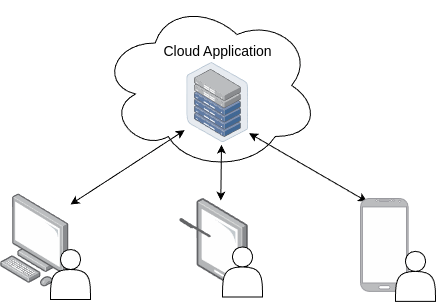
\includegraphics[scale=0.4]{images/basic-cloud-services.drawio.png}
    \caption{Cloud Application.}
    \label{fig:cloud-applications}
\end{figure}

% A key selling point of these, is that companies don't have to do any technical work setting the software up, they can pay for a subscription and start using the tool right away, either through a browser or by installing an executable on their computer.
% A very important technical aspect for such tools, that enables the ease of use, is the ability to support multiple companies using them at once.
Most of these benefits only apply if the same instance of the application is able to serve every user.
This is called multi-tenancy, and it is implemented by most popular cloud applications, e.g. by Teams, Slack, Asana, and many more.
A tenant can be seen as an entity that uses the application, which can be either a single user or an organization made up of many users.

\begin{figure}[H]
    \centering
    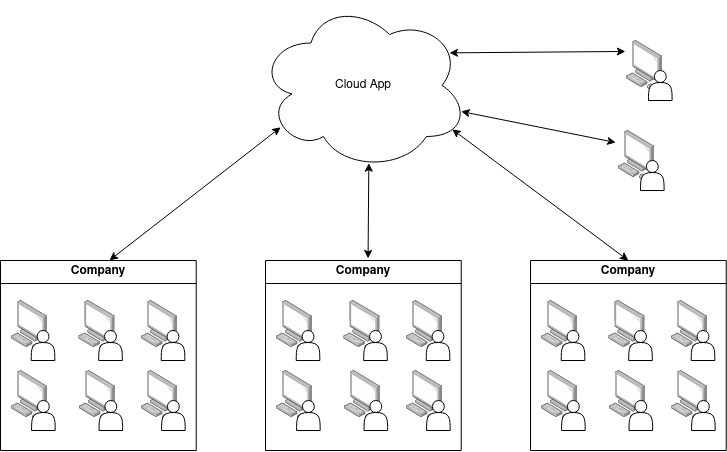
\includegraphics[scale=0.45]{images/mt-cloud-services.png}
    \caption{Multi tenancy in cloud applications.}
    \label{fig:multi-tenant=cloud-applications}
\end{figure}

PROCEED (short for PROCess EnginE in a Distributed environment) is a cloud application,
it is a decentralized Business Process Management System.
PROCEED uses BPMN at its core to model and execute business processes.
%For readers unfamiliar with BPMN, 
%it can be thought of as a powerful flowchart that can be used to describe any conceivable process.
BPMN (Business Process Model and Notation) is a standardized graphical notation used for documenting business processes.
BPMN is typically used inside of organizations to illustrate sequences of tasks,
decision points, and interactions within various business processes, providing a standardized visual representation.

PROCEED offers two products:
\begin{itemize}
    \item Distributed Process Engine (DPE): the DPEs execute bpmn processes in a distributed fashion.
    \item Management System (MS): the MS is a cloud application that gives users a graphical interface to manage their processes and deploy these to the DPEs.
\end{itemize}

\begin{figure}[H]
    \centering
    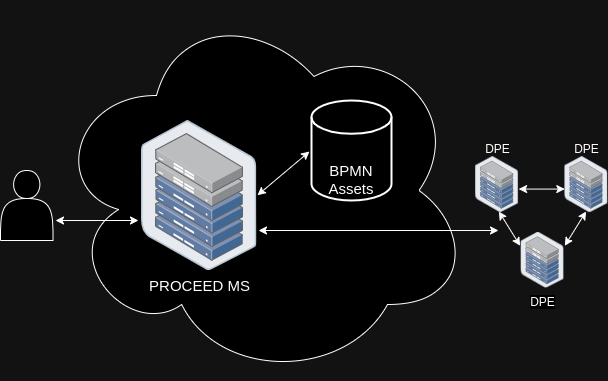
\includegraphics[scale=0.45]{images/quick-ms-overview.drawio.png}
    \caption{Overview of PROCEED.}
    \label{fig:proceed-overview}
\end{figure}

%Throughout this thesis we'll refer to any information that a user can access as an asset.
%Also all actions that a user can perform in the PROCEED Management System, are viewed as an action performed on an asset.

%The PROCEED Management system encompasses various asset types, which can be categorized as follows:
%\begin{enumerate}
%    \item BPMN models: Processes, Projects, and Templates are assets that can be created in PROCEED, that fall into the category of BPMN models.
%    Although each one of them stores slightly different information and carries a distinct semantic meanings, they all have BPMN at their core.
%    \item Execution related assets: Tasklist, Executions and Machines are all assets related to the execution of a BPMN model.
%end{enumerate}

Currently, the MS doesn't support multi-tenancy, it only supports individual users, which means that each user has only access to his assets.
For this reason, it presents many difficulties for organizations, as there is no convenient way for multiple members of the organization to work together on assets in the MS.
Furthermore, any admin user in the MS has the right to view and modify every asset, which presents privacy risks for organizations.

For these reasons, the only viable option for organizations to use PROCEED, is to spin up an instance of the MS on their own computers, which renders most benefits of cloud applications void.
%This is because all assets are stored in a central database without a good way to isolate them from other tenants.
%The only information that BPMN related assets are stored with, that helps towards isolating them from other tenants is the owner and a set of labels.

This thesis implements multi-tenant functionality into the PROCEED Management System by introducing the concept of Environments. 

Each tenant will be able to work in their isolated environment, which lives in a central instance of the Management System. 
Additionally, each account implicitly has its own Environment allowing users to work on personal projects, keeping these separated from any other users.

\begin{figure}[H]
    \centering
    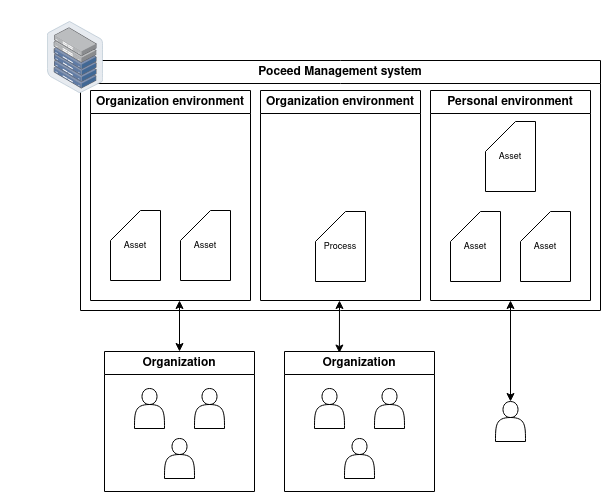
\includegraphics[scale=0.6]{images/proceed-workspaces-v2.drawio.png}
    \caption{Environments in PROCEED.}
    \label{fig:proceed-envitonments-overview}
\end{figure}

Additionally, environments will provide a more sophisticated way to manage assets. 
Currently, the MS only provides labels for organizing assets, users cannot add, delete nor modify these labels.
Environments will include a folder structures to organize BPMN assets, which provides more flexibility than labels.
% These labels symbolize, what department the process belongs to. 

%Access to assets in the MS is restricted through roles,
%so that one of three scenarios can happen to a user:
%
%\begin{itemize}
%    \item The user doesn't permissions to see assets.
%    \item The user has permission to view assets, but isn't an admin. In case, the user would only be able to see his own assets.
%    \item The user is an admin and can see all assets.
%\end{itemize}
%
%This low level of granularity makes the PROCEED Management System unsuitable hosting multiple tenants, since all their assets would be stored in the same fashion, and the only way for users to see assets that weren't created by them, would be to grant them the admin role.
%Granting users the admin role, would in turn mean that they would be able to see all BPMN Assets, which poses privacy concerns for tenants, since other tenants could potentially access their assets.

%When it comes to Execution related assets, Machines and Executions also have similar problems to BPMN assets, since these need to be private for each company.

%This makes it so, that if more than one tenant wants to use PROCEED they're left with few options:
%
%\begin{itemize}
%\end{itemize}
%Each company would have to spin up their own self hosted version of PROCEED.
%
%Both of these options have considerable downsides. 
%No separation between companies is a hindrance to privacy and each company having to spin up an instance of PROCEED is a big barrier to entry.
%This makes it very hard to scale PROCEED to be able to be comfortably used by multiple companies.
%
%\begin{figure}[H]
%    \centering
%    \includegraphics[scale=0.5]{images/PROCEED-no-Environments.drawio.png}
%    \caption{PROCEED Management System with no multi-tenant support.}
%    \label{fig:PROCEED-no-Environments}
%\end{figure}


% Research questions
\chapter{Research Questions}
\label{cha:researchquestions}


% Task List

\chapter{Task List}
\label{cha:tasklist}

% private environment
% Functional / non functional
% can / must / should 

\begin{enumerate}
  \item Functional
  \begin{enumerate}
    %TODO: I have to write everything about environments still
    \item The MS must be able to hold multiple environments and let users access them concurrently.

    \item The MS has to support two types of environments: personal and organization environments.
    \begin{enumerate}
      \item Every user has to have a personal environment, of which only he can be a member.
      %NOTE: im talking about roles here, maybe should go somewhere else
      \item Organization environments must be able to have multiple members and roles that control what each member can do.
      \item Environments must have a folder system to store assets.
      \begin{enumerate}
          \item Find a suitable abstraction to represent folders in a database.
          \item Ensure privacy between environments.

          escribir aca ya que tiene que haber herencia
          reescribir should be modified no es tan fuerte/
          \item Existing access managemnt has to be adapted to fit folders: Currently in the MS, conceptually, all Assets are stored in one folder, and access rules apply to each element of this folder.
            With a new folder structure, how roles act on different resources should be modified, depending on what folder the resources are in.
      \end{enumerate}
    \end{enumerate}

    \item Environments must be isolated from each other, so that users can only access assets in environments they are members of.

    %NOTE: maybe carry out actions no the best frasing
    \item Users must be able to be members of multiple environments and carry out actions in each one of them.

    \item The MS's preexisting role system must be adapted to fit environments:
      The proceed management system already has a role system in place to manage user's access to resources, these roles need to be modified for them to work with environments.
    \begin{enumerate}
        \item Ensure roles are always enforced in the backend.
        \item The frontend UI must adapt to a user's roles, by only showing options that the user has permission to do.
    \end{enumerate}

  \end{enumerate}

  \item Non functional
  \begin{enumerate}
    \item Try to keep changes to the existing codebase to a minimum.

    \item The same data structure should be used for both personal and organization environments.

    % \item The implentation shoudln't be repetitive, the same functional components should be used for both personal and organization environments.

    \item The user interface for navigating folders should be intuitive.

    \item Implement environments in a way that enables a good developer experience.
    \begin{enumerate}
        % not functional 
        \item Create simple abstractions for the backend code of the MS, that allow to acknowledge a user's environment with minimal effort.
        \item Create a simple abstraction for the frontend, that makes it so, that the frontend doesn't need to know what environment the user belongs to.
    \end{enumerate}
  \end{enumerate}
    \item Environments should be easy to create, manage and delete.
    \begin{enumerate}
        \item The frontend should provide intuitive interfaces for creating and deleting organization environments.
        // not functional
        \item Provide well documented APIs to create, manage and delete environments both for the frontend and the backend.
        needs more description. ldap
        \item Environments should provide the option to import an existing user database.
    \end{enumerate}

\end{enumerate}


%---------------- 
% old

% \begin{enumerate}
    % \item The same data structure should be used to represent personal and organization environments.
    % \begin{enumerate}
        % \item Personal and organization environments should have a near identical structure.
        % kann man falsch verstehen umschreiben
        % \item Most of the backend and frontend code should work the same, regardless of if it is dealing with a personal or an organization environment.
    % \end{enumerate}

    % not functional - keine stichpunkte  - : 2 points in one paragraph

% \end{enumerate}

% The introduction of "environments" within this system is a pivotal enhancement. These environments serve as distinct, isolated spaces, ensuring that the contents and operations within each environment remain entirely separate from those in all other environments. This separation offers users the capability to manage various aspects of PROCEED's functionality while maintaining data and process integrity within their designated environment. This thesis explores the design, implementation, and implications of the multi-tenant feature within the Management System of Proceed, contributing to a more versatile and secure user experience.
